\section{模型验证与敏感性摘要}
\label{sec:validation}

四问共用同一求解器，验证从独立解析解、离散收敛、守恒和结构性退化四个层面进行。问题一常物性温度方程的 Bessel--Duhamel 解与数值解最大偏差为 $5.224\times10^{-4}$ °C；问题三、四在 $N=160$ 时均满足相邻网格相对差不超过 $5\times10^{-4}$，而 $\Delta t$ 从 $4$ s 减至 $0.5$ s 仅使 $t_{\mathrm{dry}}$ 改变约 $3\times10^{-3}$ h。零输入、常空气解析、纯扩散守恒和收缩关闭四项退化检验均通过；四问守恒残差为 $10^{-11}\sim10^{-10}$。完整判据、逐档数据与图表见附录 C。

单因子重算表明，烘干时长的敏感性顺序为
\begin{equation}
R(t)\gg h_m>T_{\mathrm{air}}\gg W_{\mathrm{air}}\gg h.
\end{equation}
其中半径 $\pm5\%$ 引起约 $\pm9\%$ 的时长变化，中心差商弹性为 $1.810$；$h_m$ 减少 $20\%$ 使时长增加 $2.973\%$，而 $h$ 的双向扰动仅约 $\pm0.03\%$。这说明全过程由传质与几何尺度控制，未显式计入汽化潜热会影响表面温度估计，但不是时长的主导不确定度。两种烘干时长分别为 $2.3927$ d 和 $2.1280$ d，均位于题设给出的 $2$--$3$ d 先验区间内。

\begin{figure}[!htbp]
\centering
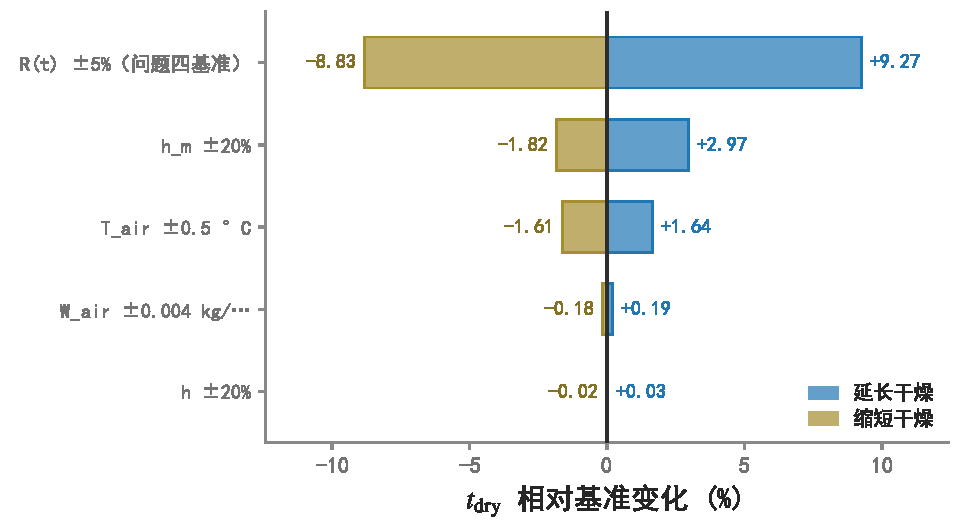
\includegraphics[width=.62\textwidth,height=.35\textheight,keepaspectratio]{../figures/fig_sensitivity_tornado.pdf}
\caption{单因子灵敏度排序}
\label{fig:sensitivity_tornado}
\end{figure}
